% This is samplepaper.tex, a sample chapter demonstrating the
% LLNCS macro package for Springer Computer Science proceedings;
% Version 2.20 of 2017/10/04
%
\documentclass[runningheads]{llncs}

\usepackage{geometry}
\geometry{
  a4paper,         % or letterpaper
  textwidth=15cm,  % llncs has 12.2cm
  textheight=24cm, % llncs has 19.3cm
  heightrounded,   % integer number of lines
  hratio=1:1,      % horizontally centered
  %vratio=2:3,      % not vertically centered
}

%%
\usepackage{graphicx}
\usepackage{floatrow}
\usepackage[title]{appendix}
\usepackage{listings}
\lstset{language=Python}          % Set your language (you can change the language for each code-block optionally)
\usepackage{color}


% Table float box with bottom caption, box width adjusted to content
\newfloatcommand{capbtabbox}{table}[][\FBwidth]

\begin{document}
	
\definecolor{dkgreen}{rgb}{0,0.6,0}
\definecolor{gray}{rgb}{0.5,0.5,0.5}
\definecolor{mauve}{rgb}{0.58,0,0.82}

\lstset{frame=tb,
	language=Java,
	aboveskip=3mm,
	belowskip=3mm,
	showstringspaces=false,
	columns=flexible,
	basicstyle={\small\ttfamily},
	numbers=none,
	numberstyle=\tiny\color{gray},
	keywordstyle=\color{blue},
	commentstyle=\color{dkgreen},
	stringstyle=\color{mauve},
	breaklines=true,
	breakatwhitespace=true,
	tabsize=3
}
	
%
\title{Assignment-3 of Deep Learning in Computer Vision}
\subtitle{Generative Adversarial Networks}
%
%\titlerunning{Abbreviated paper title}
% If the paper title is too long for the running head, you can set
% an abbreviated paper title here
%
\author{Xiao Hu\inst{1} \and
Boya Wu\inst{2}}

\institute{
%\email{xiahaa@space.dtu.dk} \and
%{} \and
%\\\
%\url{http://www.springer.com/gp/computer-science/lncs} \and \\
1. \email{xiahaa@space.dtu.dk},\ 2. \email{s170061@student.dtu.dk}}
%
\maketitle              % typeset the header of the contribution
%
% \begin{abstract}
% The abstract should briefly summarize the contents of the paper in
% 150--250 words.

% \keywords{\textbf{NO MORE THAN 6 PAGES}  \and Second keyword \and Another keyword.}
% \end{abstract}
%
%\section{Introduction}
\section{Generation of MNIST digits with a GAN}
We have investigated a Generative Adversarial Networks (GAN) problem by generating digits in the MNIST-like fashion. The following tasks have been done:
\begin{itemize}
    \item Implement a GAN as fully connected neural network and generate MNIST-like digits using Vanilla loss.
    \item Generate MNIST-like digits using least square loss.
    \item Implement DCGAN and generate MNIST-like digits.
    \item Implement cGAN and generate MNIST-like digits.
    \item Implement a cGAN that transform from SVHN to MNIST-like digits.
\end{itemize}

\subsection{GAN Design}
For GAN, shown in Figure~\ref{fig1} :
\begin{itemize}
	\item Generator: $4$ fully connected layers with leaky ReLU (slope$=0.1$) and batch normalization. Finally, the output is reshaped to a $28\times 28$ image and apply tanh to each pixel.
	\item Discriminator: $4$ fully connected layers with hidden units being $1024,\ 512,\ 256,\ 1$. Drouout is added after each fully connected layer.
\end{itemize}
For DCGAN, shown in Figure~\ref{fig2} :
\begin{itemize}
	\item Generator: $4$ deconvolution layers with leaky ReLU (slope$=0.1$) and batch normalization followed by $1$ convolution layer and use tanh to make each pixel ranging from $-1$ to $1$.. Feature channels are $1024,\ 512,\ 256,\ 128$. 
	\item Discriminator: $4$ convolution layers with feature channels being $128,\ 256,\ 512,\ 1$. The first three convolution layers are cascaded with a leaky ReLU (slope$=0.1$) and dropout.
\end{itemize}
\begin{figure}[ht]
	\centering
	\setlength{\fboxrule}{0.0pt}
	\framebox{\parbox{2.8in}{
			\centering
			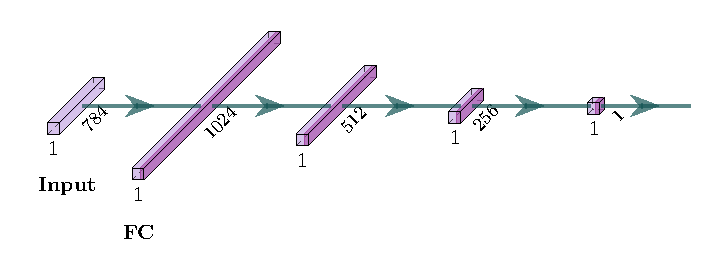
\includegraphics[width=.45\textwidth]{figures/gan_dis}
	}}
	\framebox{\parbox{2.8in}{
			\centering
			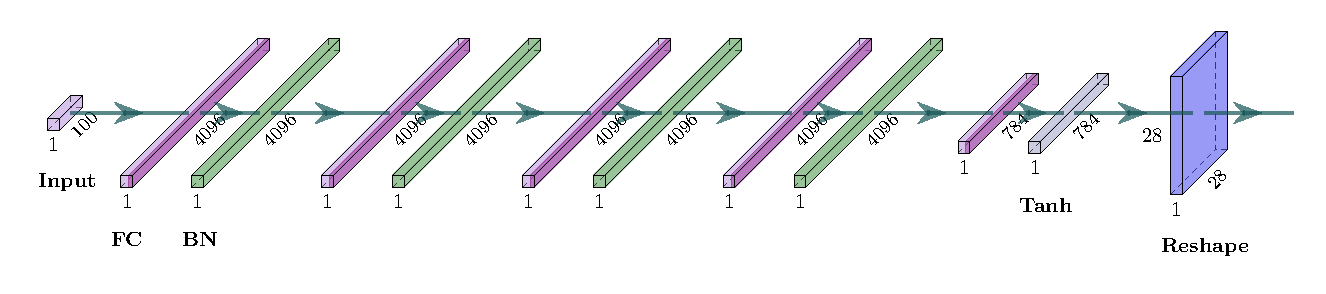
\includegraphics[width=.45\textwidth]{figures/gan_gen}
	}} 
	\caption{GAN: discriminator (left) and Generator (right).}
	\label{fig1}
\end{figure}
\begin{figure}[ht]
	\centering
	\setlength{\fboxrule}{0.0pt}
	\framebox{\parbox{2.8in}{
			\centering
			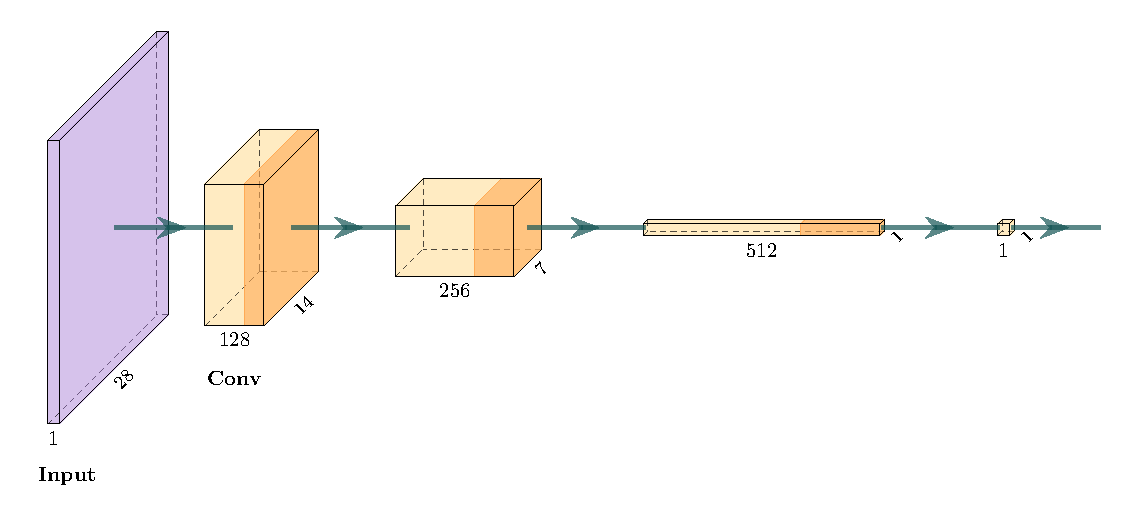
\includegraphics[width=.45\textwidth]{figures/dcgan_dis}
	}}
	\framebox{\parbox{2.8in}{
			\centering
			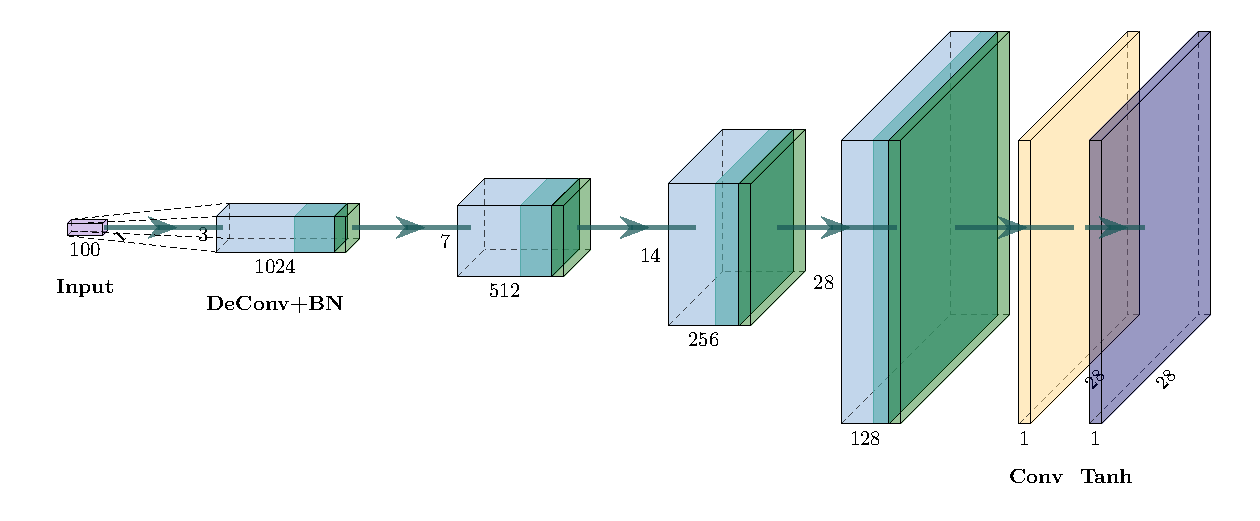
\includegraphics[width=.45\textwidth]{figures/dcgan_gen}
	}} 
	\caption{DCGAN: discriminator (left) and Generator (right).}
	\label{fig2}
\end{figure}

\subsection{Result} 
\subsubsection{GAN+Vanilla Loss} Result after $10$ epochs training is shown in the left image of Figure~\ref{fig3}.
\subsubsection{GAN+Least Square Loss} Result after $10$ epochs training is shown in the middle image of Figure~\ref{fig3}.
\begin{figure}[ht]
	\centering
	\setlength{\fboxrule}{0.0pt}
	\framebox{\parbox{1.8in}{
			\centering
			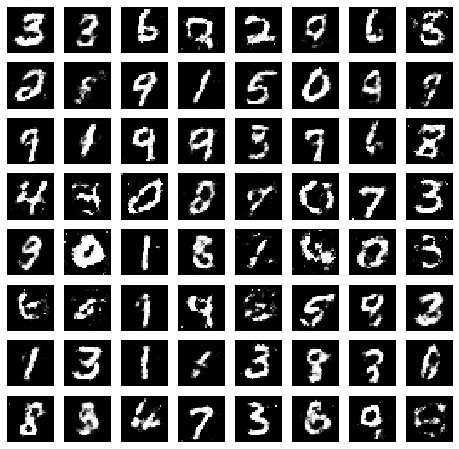
\includegraphics[width=.3\textwidth]{figures/vanila_gan_0_9.png}
	}}
	\framebox{\parbox{1.8in}{
			\centering
			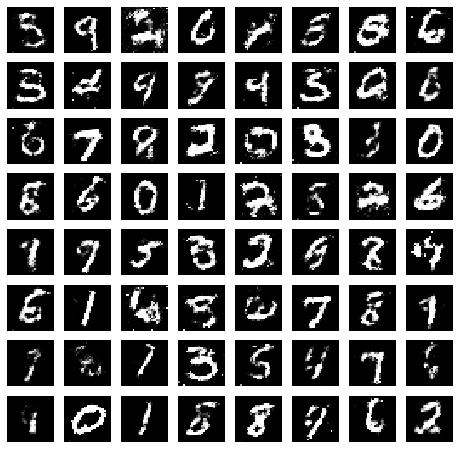
\includegraphics[width=.3\textwidth]{figures/ls_gan_0_9.png}
	}} 
	\framebox{\parbox{1.8in}{
		\centering
		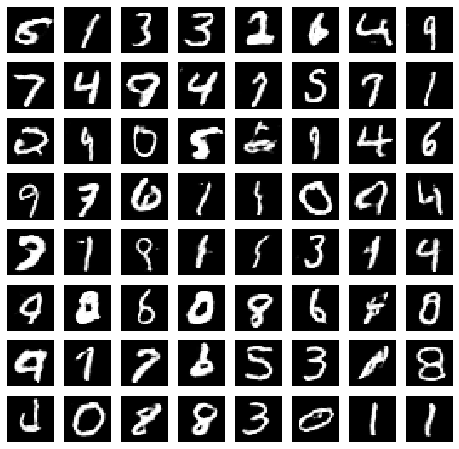
\includegraphics[width=.3\textwidth]{figures/dcgan_0_9.png}
}} 
	\caption{Faked MNIST images generated by GAN+Vanilla loss (left), GAN+least square loss (middle), and DCGAN(right).}
	\label{fig3}
\end{figure}
\subsubsection{DCGAN+Least Square Loss} Result after $10$ epochs training is shown in the right image of Figure~\ref{fig3}.

It can be seen DCGAN outperforms GAN. As a result, for the following parts, we keep using DCGAN and least square loss function.

\begin{figure}[ht]
	\centering
	\setlength{\fboxrule}{0.0pt}
	\framebox{\parbox{2.8in}{
			\centering
			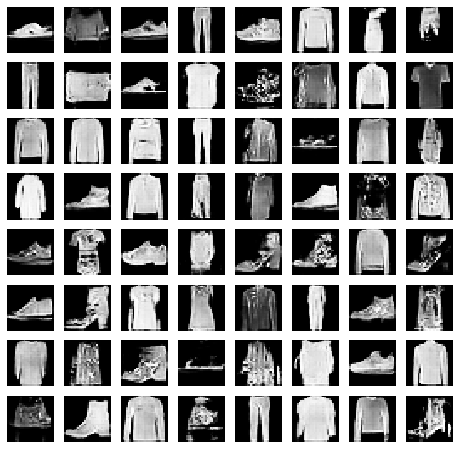
\includegraphics[width=.4\textwidth]{figures/dcgan_fashion_mnist.png}
	}}
	\framebox{\parbox{2.8in}{
			\centering
			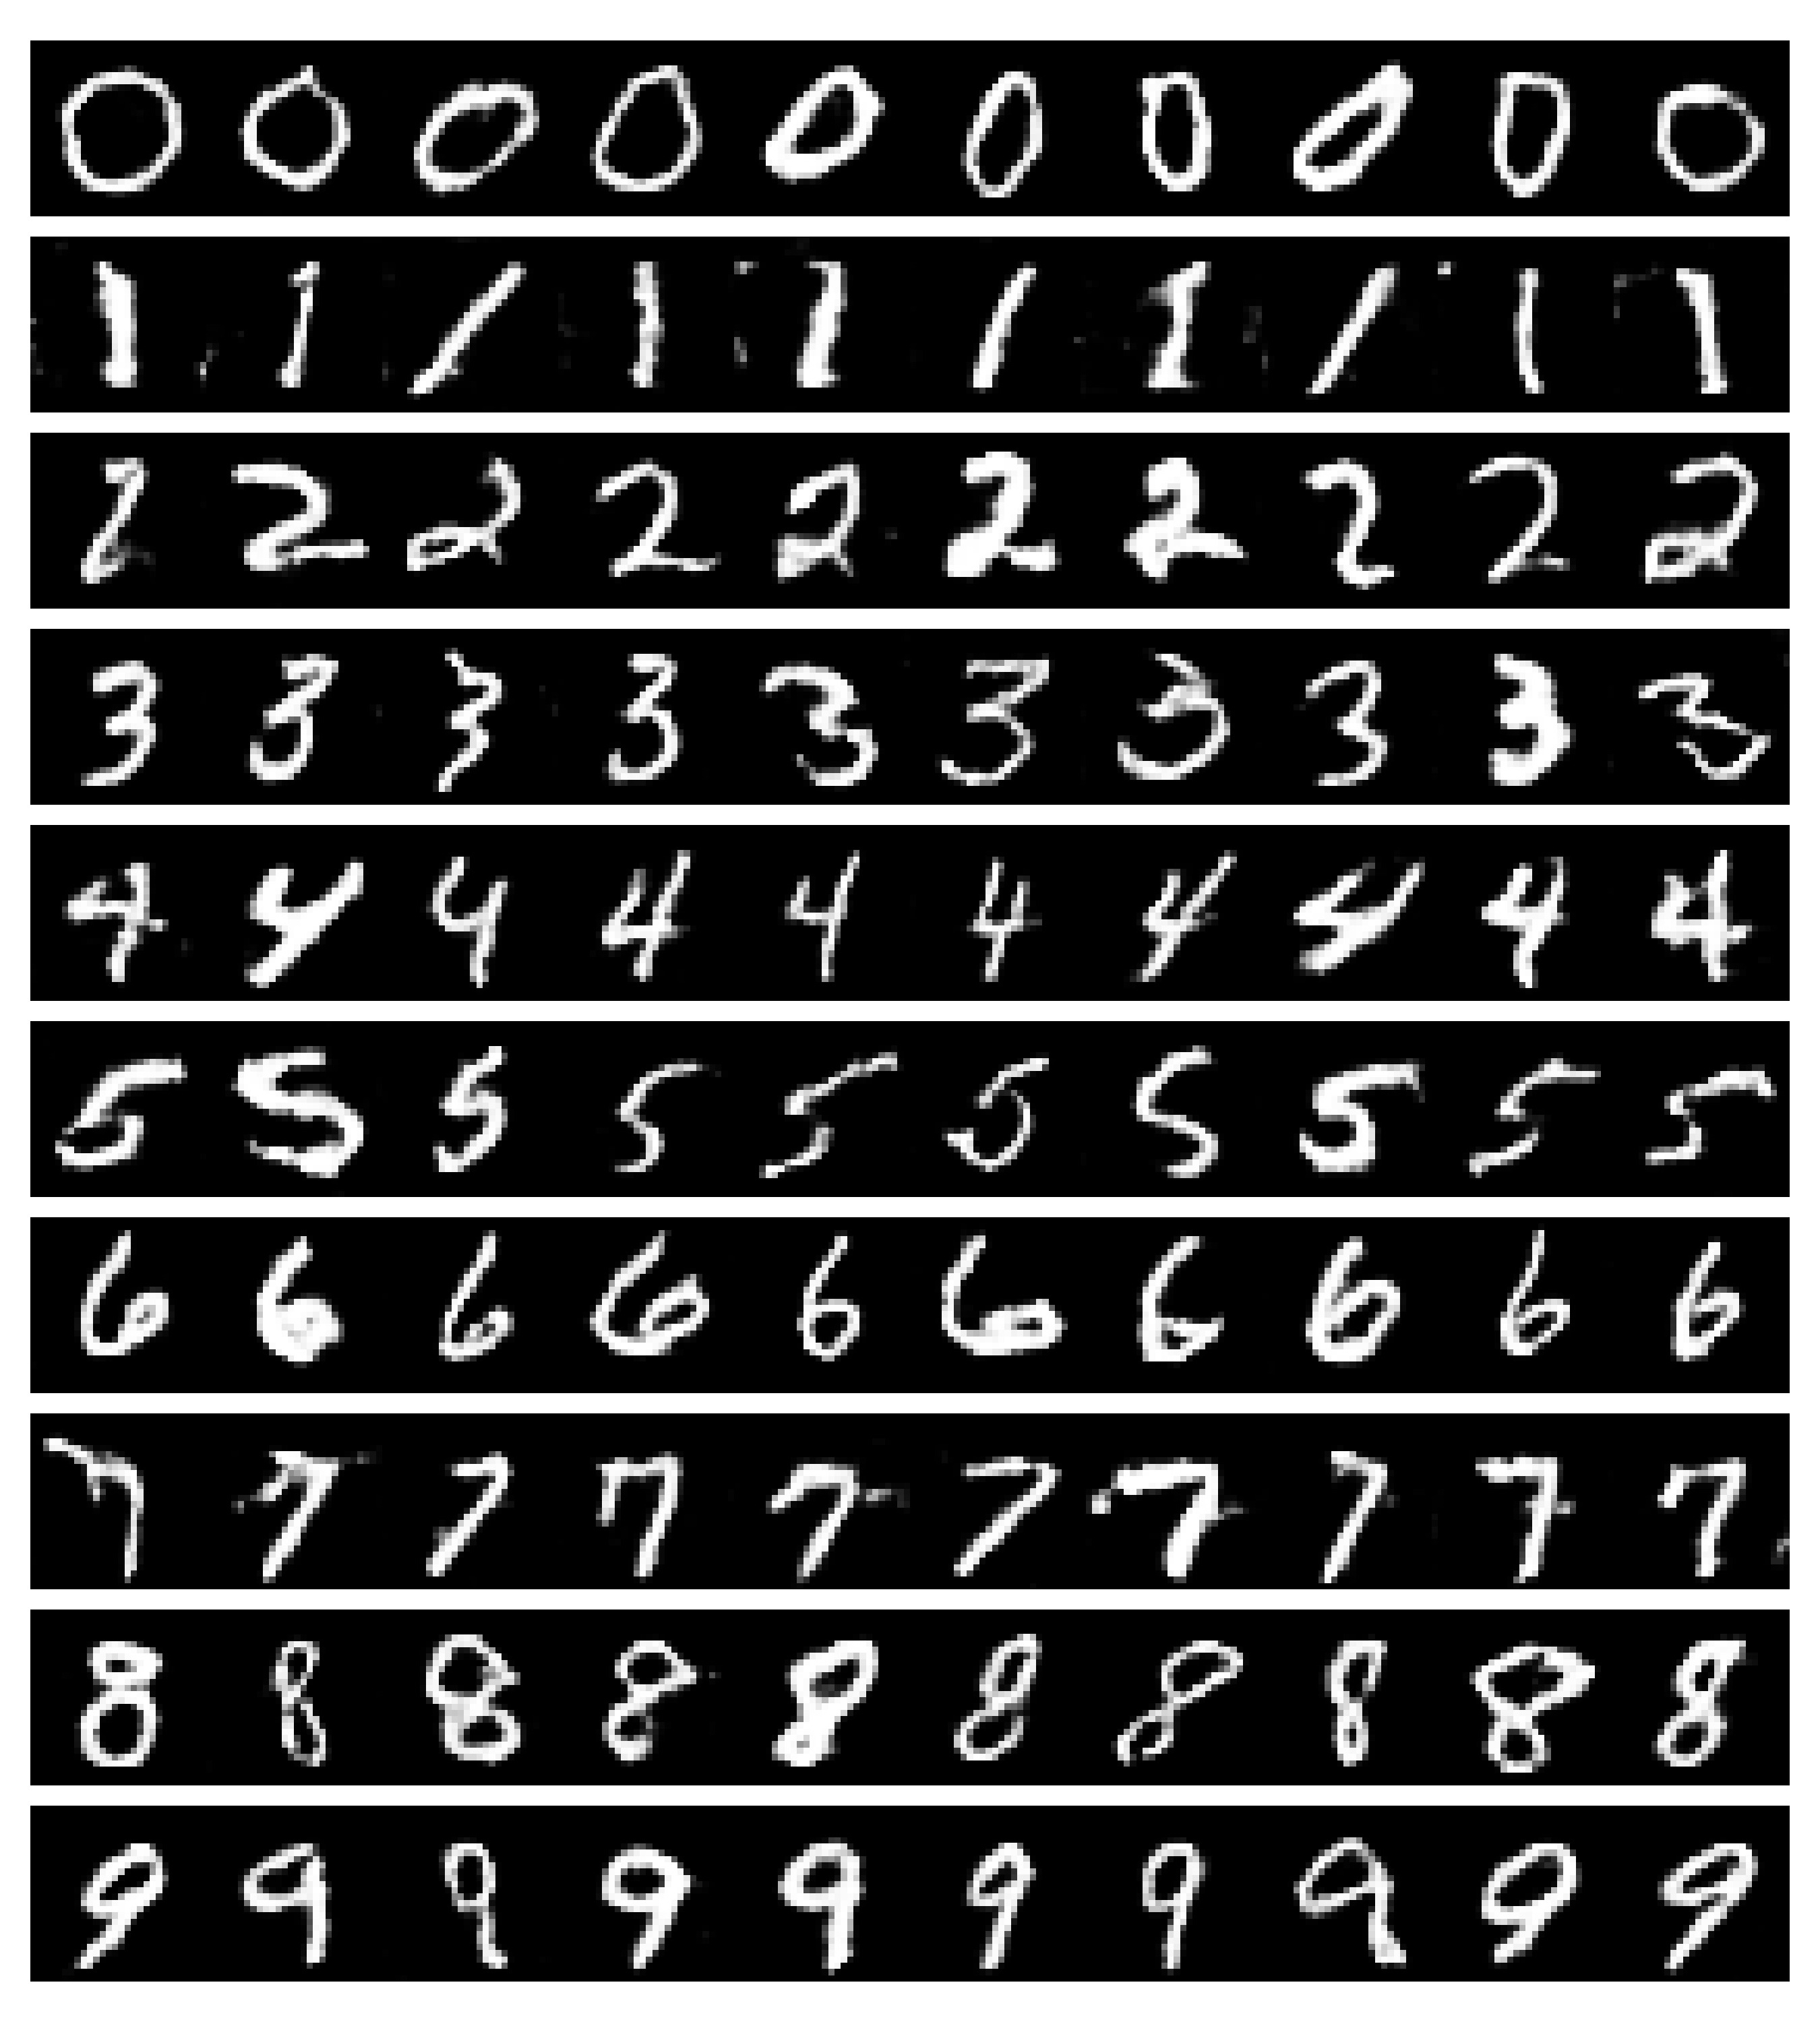
\includegraphics[width=.4\textwidth]{figures/cgan_0_9.png}
	}} 
	\caption{Faked FashionMNIST images generated by DCGAN+least square loss (left) and cGAN (right).}
	\label{fig4}
\end{figure}

\subsubsection{DCGAN+FashionMNIST} We applied the implemented DCGAN on FashionMNIST dataset. This time, the length of the random vector is increased to $300$ since the dimension of the embedded manifold of FashionMNIST is higher than that of MNIST. Result after $10$ epochs training is shown in the left image of Figure~\ref{fig4}. It can be seen that the DCGAN is able to generate images in FashionMNIST style. However, compared with raw FashionMNIST images, it still misses some detailed texture. Training with more epochs or use higher dimension random vector may be helpful to get better result.

\subsubsection{cGAN} We use DCGAN to implement the conditional GAN. Result after $10$ epochs training is shown in the right image of Figure~\ref{fig4}. For each row, we draw the sample label and generated $10$ samples.

\subsubsection{cGAN+SVHN} We use the implemented cGAN to transform from SVHN digits to MNIST digits. Result is shown in Figure~\ref{fig5}. For each row, we randomly select $10$ samples from SVHN dataset and then transform to MNIST style.
\begin{figure}[ht]
	\centering
	\setlength{\fboxrule}{0.0pt}
	\framebox{\parbox{2.8in}{
			\centering
			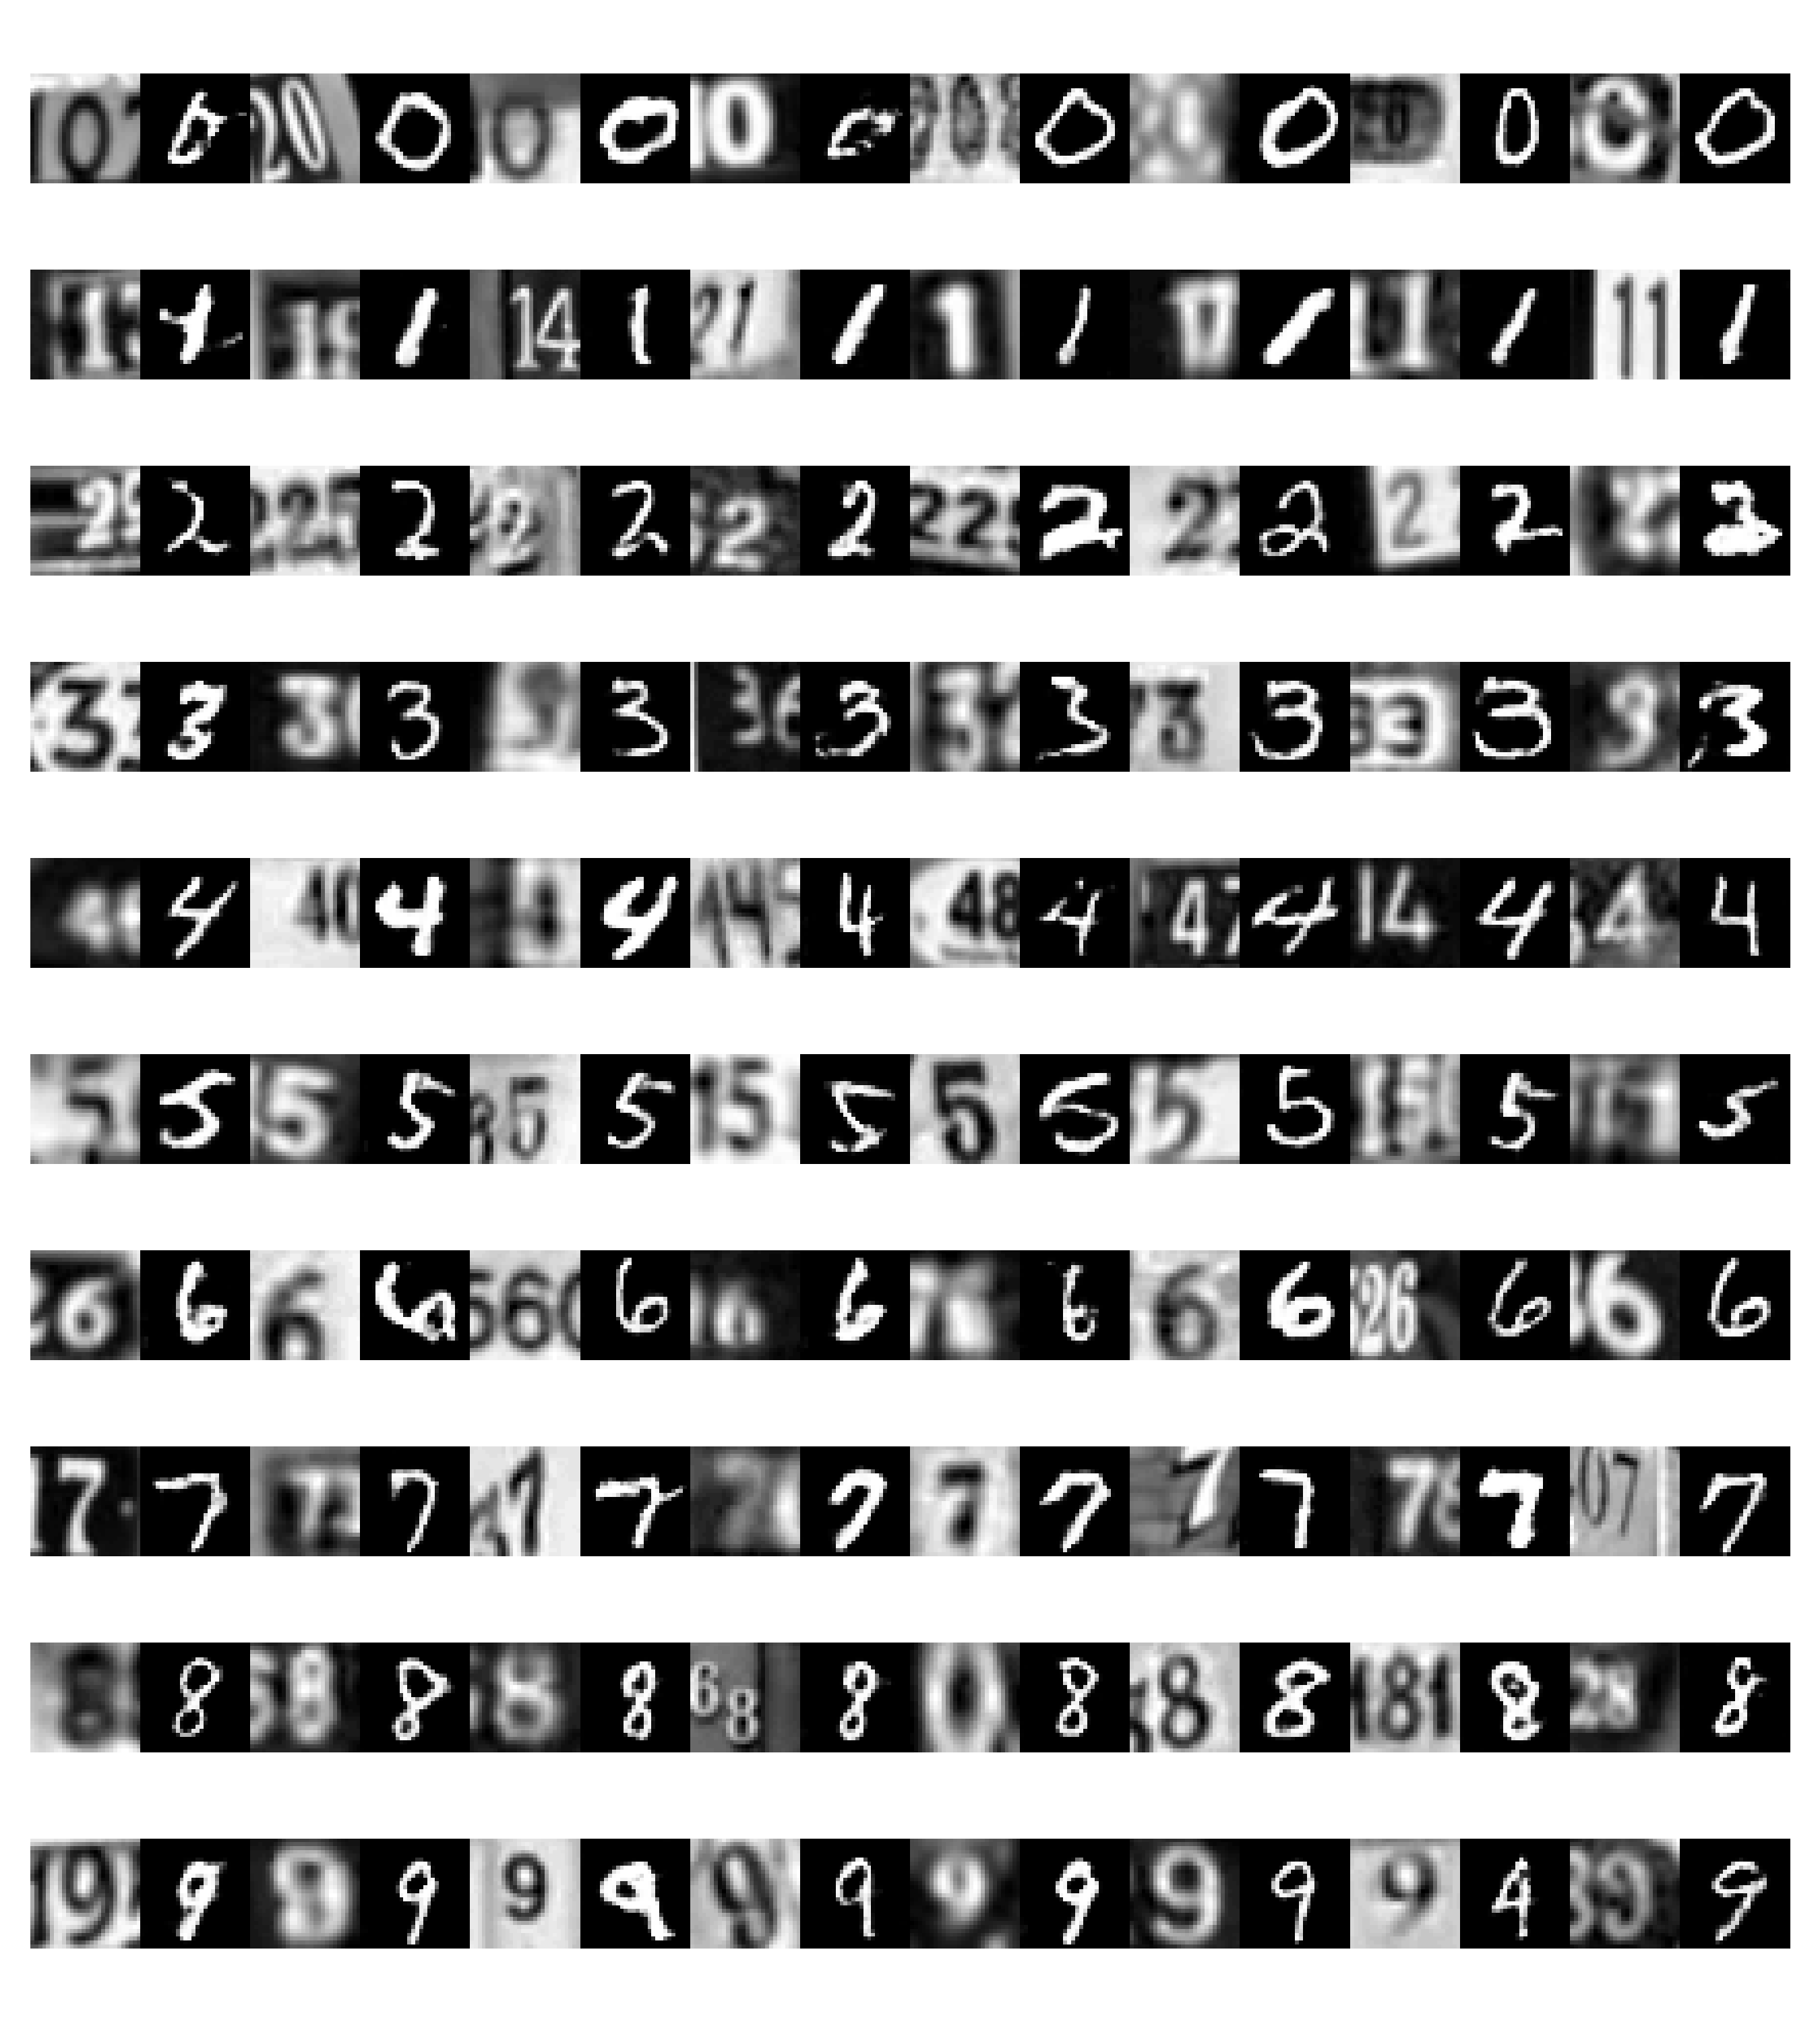
\includegraphics[width=.6\textwidth]{figures/svhn_0_9.png}
	}}
	\caption{Style transfer from SVHN images to MNIST images.}
	\label{fig5}
\end{figure}




\section{CycleGAN}
The second task is to implement a CycleGAN to convert horses to zebras and vice versa. The following tasks have been done:
\begin{itemize}
	\item Implement a CycleGAN.
	\item Train CycleGAN for image translation between horses and zebras.
\end{itemize}

\subsection{CycleGAN Network}
The generator and discriminator for cycleGAN are shown in Figure~\ref{fig7}.
\begin{figure}[ht]
	\centering
	\setlength{\fboxrule}{0.0pt}
	\framebox{\parbox{2.8in}{
			\centering
			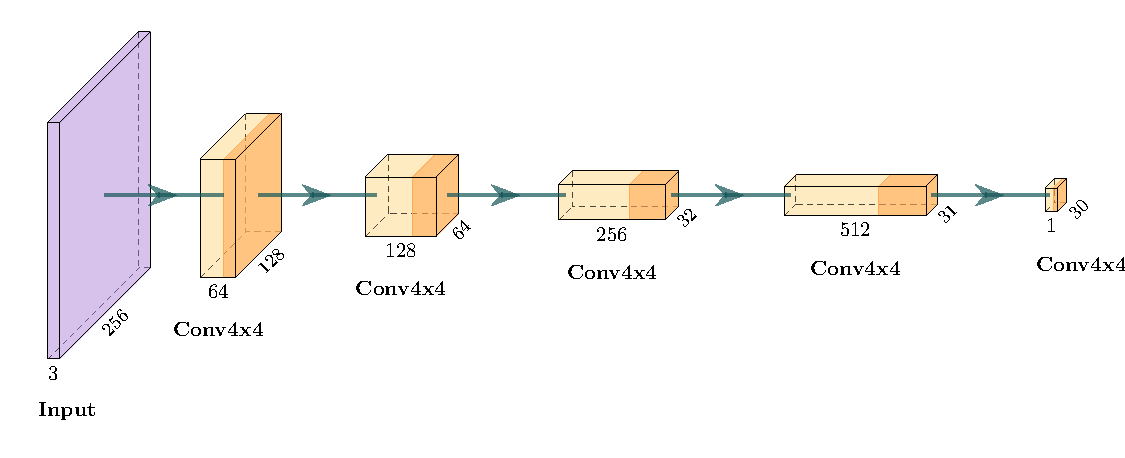
\includegraphics[width=.45\textwidth]{figures/netcyclegan_dis}
	}}
	\framebox{\parbox{2.8in}{
			\centering
			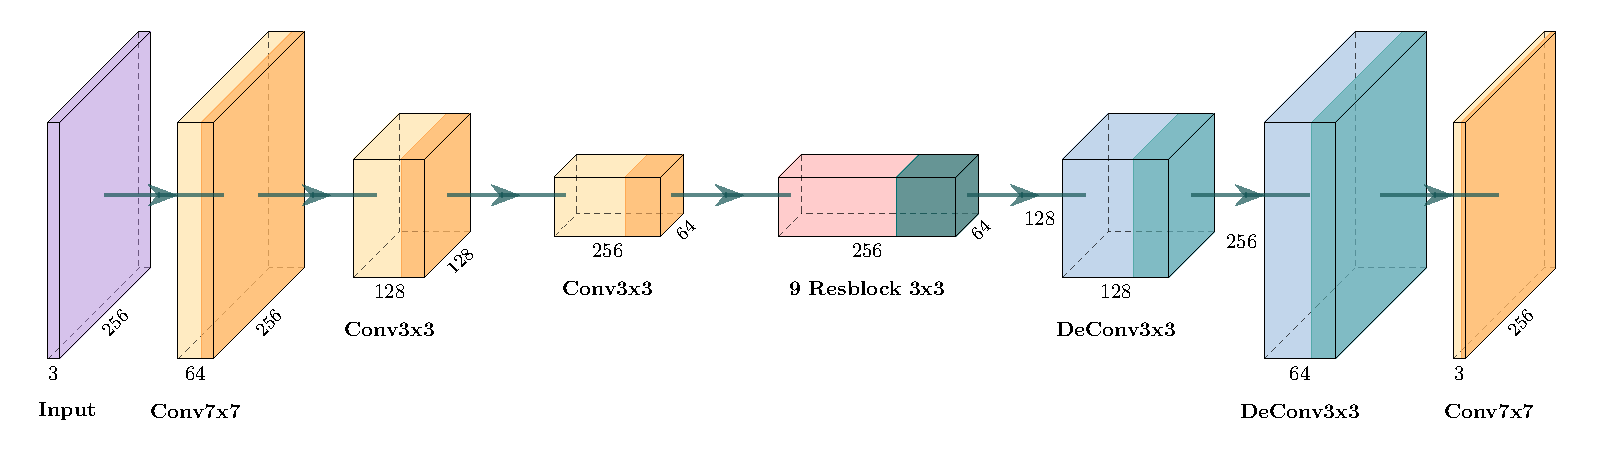
\includegraphics[width=.45\textwidth]{figures/netcyclegan_gen}
	}} 
	\caption{CycleGAN: discriminator (left) and Generator (right).}
	\label{fig7}
\end{figure}
For building up CycleGAN, we actually need two generators: $G_{A\to B}$, $G_{B\to A}$, and two discriminator: $D_{A}$, $D_{B}$. 

\subsection{Loss Function}
Three types of loss are needed:
\begin{itemize}
	\item GAN loss: here we use least square GAN loss.
	\item Identity loss: e.g. $|G_{A\to B}(a_{real})-a_{real}|$, $L_{1}$ norm is used here.
	\item Cycle loss: e.g $|G_{B\to A}(G_{A\to B}(a_{real}))-a_{real}|$, $L_{1}$ norm is used here.
\end{itemize}
The final loss is the combination of the three loss:
$$
loss_{total}=loss_{GAN}+\lambda_1 loss_{ind} + \lambda_2 loss_{cycle}
$$
$\lambda_1=0.5$, $\lambda_2=10$ are used here. 

\subsection{Training}
Since training CycleGAN is really time consuming, we have not been able to train our network more than 10 epochs due to the time limitation. The result after $2$ epochs is shown in 
\begin{figure}[ht]
	\centering
	\setlength{\fboxrule}{0.0pt}
	\framebox{\parbox{5.8in}{
			\centering
			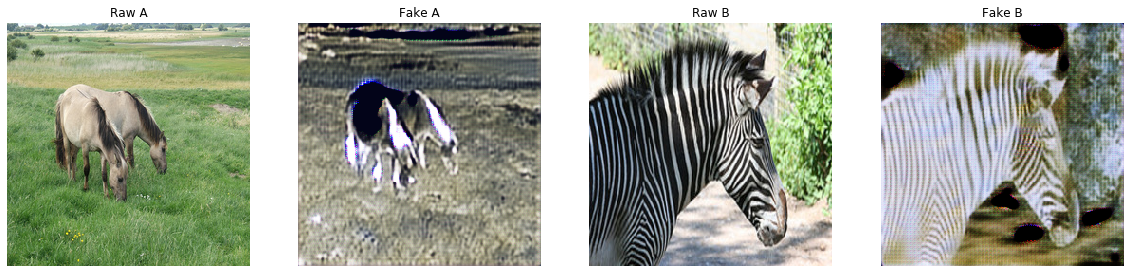
\includegraphics[width=.95\textwidth]{figures/cyclegan.png}
	}}
	\caption{CycleGAN result after 2 epochs.}
	\label{fig7}
\end{figure}
We can see there are indeed some style tranfer effects. However, it is far from perfection. We think use more epochs may generate more promissing result.

\subsection{Analysis}
From the CycleGAN paper, right), there is an assumption that ``We assume there is some underlying relationship between the domains – for example, that they are two different renderings of the same underlying scene – and seek to learn that relationship.'' Thus, we think the more diverged the scene is, the bad the performance of CycleGAN will be.



\begin{subappendices}
	\renewcommand{\thesection}{\Alph{section}}%
	% or try \arabic{section}
	
	\section{Generator \& Discriminator}
\begin{lstlisting} 
class ResNetBlock(nn.Module):
	def __init__(self, n_features):
		super(ResNetBlock, self).__init__()
		self.resblock = nn.Sequential(
		nn.Conv2d(n_features,n_features,kernel_size=3,
		stride=1,padding=(1,1)),
		nn.InstanceNorm2d(n_features),
		nn.ReLU(),
		nn.Conv2d(n_features,n_features,kernel_size=3,stride=1,padding=(1,1))
		)

	def forward(self, x):
		out = self.resblock(x);
		out+=x
		out = F.relu(out) ## could use leaky_relu?
		return out
\end{lstlisting}

\begin{lstlisting} 
def deconv(c_in, c_out, k_size, stride=2, padding=1, output_padding=0, bias = True, insn=True, relutype = 1, alpha=0.2):
	'''
	return deconvolusion layers
	'''
	layers = []
	layers.append(nn.ConvTranspose2d(c_in, c_out, k_size, stride, padding, bias=bias, output_padding=output_padding))

	if relutype == 1:
		layers.append(nn.LeakyReLU(alpha))
	else:
		layers.append(nn.ReLU())
	
	if insn:
		layers.append(nn.InstanceNorm2d(c_out))
	return nn.Sequential(*layers)

def conv(c_in, c_out, k_size, stride=2, padding=1, bias = True, insn=True, relutype = 1, alpha=0.2):
	'''
	return convolution layers
	'''    
	layers = []
	layers.append(nn.Conv2d(c_in, c_out, k_size, stride, padding, bias=bias))
	if relutype == 1:
		layers.append(nn.LeakyReLU(alpha))
	else:
		layers.append(nn.ReLU())

	if insn:
		layers.append(nn.InstanceNorm2d(c_out))
	return nn.Sequential(*layers)
\end{lstlisting}

\begin{lstlisting} 
class G(nn.Module):
	'''
	generator
	'''
	def __init__(self, input_features = 3, output_features = 3):
		super(G, self).__init__()
		# encoding blocks
		features = 64
		self.conv1 = conv(input_features, features, 7, stride=1, padding=3,relutype=2)
		self.conv2 = conv(features, features*2, 3, stride=2,padding=1,relutype=2)
		self.conv3 = conv(features*2, features*4, 3, stride=2,padding=1,relutype=2)  # 64 x 64 x256
		
		# residual blocks
		num_res_blocks = 9
		res_layers = []
		for i in range(num_res_blocks):
			res_layers.append(ResNetBlock(features*4))
		self.res_blocks = nn.Sequential(*res_layers)
		
		# decoding blocks
		self.deconv1 = deconv(features*4, features*2, 3, stride = 2, padding = 1, output_padding=1,relutype=2)
		self.deconv2 = deconv(features*2, features, 3, stride = 2, padding = 1, output_padding=1,relutype=2)
		self.conv4 = conv(features, output_features, 7, stride = 1, padding = 3,relutype=2)

	
	def forward(self, x):
		out = self.conv1(x)      # (?, 64, 256, 256)
		out = self.conv2(out)    # (?, 128, 128, 128)
		out = self.conv3(out)      # (?, 256, 64, 64)

		out = self.res_blocks(out)
		
		out = self.deconv1(out)  # (?, 128, 128, 128)
		out = self.deconv2(out)  # (?, 64, 256, 256) F.leaky_relu(
		out = torch.tanh(self.conv4(out))              # (?, 3, 256, 256)
		return out
\end{lstlisting}

\begin{lstlisting} 
class D(nn.Module):
	"""Discriminator for mnist."""
	def __init__(self, input_features = 3, output_features = 1):
		super(D, self).__init__()
		conv_dim = 64
		self.conv1 = conv(input_features, conv_dim, 4, stride=2, padding=1, insn=False) ## 64x128
		self.conv2 = conv(conv_dim, conv_dim*2, 4, stride=2, padding=1,insn=True) ## 128x64
		self.conv3 = conv(conv_dim*2, conv_dim*4, 4, stride=2, padding=1,insn=True) ## 256x32
		self.conv4 = conv(conv_dim*4, conv_dim*8, 4, stride=1, padding=1,insn=True) ## 512x31
		
		## patch gan
		self.conv5 = conv(conv_dim*8, output_features, 4, stride=1, padding=1,insn=True) # 1x30
		#         self.conv6 = conv(output_features, output_features, 30, stride=1, padding=0) # 1x1

	def forward(self, x):
		out = self.conv1(x)    # (?, 64, 128, 128)
		out = self.conv2(out)  # (?, 128, 64, 64)
		out = self.conv3(out)  # (?, 256, 32, 32)
		out = self.conv4(out)  # (?, 512, 31, 31)
		out = self.conv5(out)  # (?, 1, 30, 30)
		#         out = self.conv6(out).squeeze() # (?,1,1,1)
		return out
\end{lstlisting}

\section{Training}
\begin{lstlisting}
	def lsgan_loss_d(dx, dz):
		b = 1
		return 0.5*torch.mean((dx - b)**2)+0.5*torch.mean((dz)**2)
	
	def lsgan_loss_g(dz):
		c = 1
		return 0.5*torch.mean((dz-c)**2)
\end{lstlisting}

\begin{lstlisting}
A_loader = horse_loader
B_loader = zebra_loader

beta1 = 0.5
beta2 = 0.9
lr = 0.0002

gA2B = G()
gB2A = G()
dA = D()
dB = D()

g_params = list(gA2B.parameters()) + list(gB2A.parameters())

g_optimizer = torch.optim.Adam(g_params, lr, [beta1, beta2])
da_optimizer = torch.optim.Adam(dA.parameters(), lr, [beta1, beta2])
db_optimizer = torch.optim.Adam(dB.parameters(), lr, [beta1, beta2])


gA2B.to(device)
gB2A.to(device)
dA.to(device)
dB.to(device)

A_iter = iter(A_loader)
B_iter = iter(B_loader)
\end{lstlisting}

\begin{lstlisting}
iter_per_epoch = min(len(A_iter), len(B_iter))

# sampling image
fixed_A = A_iter.next()[0].to(device)
fixed_B = B_iter.next()[0].to(device)

visualization = ipywidgets.Output()
display.display(visualization)
with visualization:
	plt.figure(figsize=(20,20))
	subplots = [plt.subplot(1, 4, k+1) for k in range(4)]

criterion_cycle = torch.nn.L1Loss()
criterion_identity = torch.nn.L1Loss()

epochs = 30
for epoch in tqdm(range(epochs)): 
	A_iter = iter(A_loader)
	B_iter = iter(B_loader)
	for step in tqdm(range(iter_per_epoch)):
		# load data
		imgA, label_A = A_iter.next() 
		imgA, label_A = imgA.to(device), label_A.to(device)

		imgB, label_B = B_iter.next() 
		imgB, label_B = imgB.to(device), label_B.to(device)

		
		#============ train D ============#
		# train with real images
		d_optimizer.zero_grad()
		outAA = dA(imgA)
		with torch.no_grad(): 
		outBA = dA(gB2A(imgB))
		da_gan_loss = lsgan_loss_d(outAA,outBA)
		
		outBB = dB(imgB)
		with torch.no_grad(): 
		outAB = dB(gA2B(imgA))
		db_gan_loss = lsgan_loss_d(outBB,outAB)
		
		da_gan_loss.backward()
		db_gan_loss.backward()
		d_optimizer.step()
		
		#============ train G ============#
		g_optimizer.zero_grad()
		
		# Identity loss
		loss_id_A = criterion_identity(gB2A(imgA), imgA)
		loss_id_B = criterion_identity(gA2B(imgB), imgB)
		loss_identity = (loss_id_A + loss_id_B) / 2
		
		# add cycle loss
		fake_B = gA2B(imgA)
		g_gan_loss_A = lsgan_loss_g(dB(fake_B))
		rec_A = gB2A(fake_B)
		loss_cycle_A = criterion_cycle(rec_A, imgA)
		#         g_cycle_loss = torch.mean((rec_A-imgA)**2)
		fake_A = gB2A(imgB)
		g_gan_loss_B = lsgan_loss_g(dA(fake_A))
		rec_B = gA2B(fake_A)
		loss_cycle_B = criterion_cycle(rec_B, imgB)
		
		loss_cycle = (loss_cycle_A + loss_cycle_B) / 2
		loss_GAN = (g_gan_loss_A+g_gan_loss_B)/2
		
		# Total loss
		g_loss = loss_GAN + 10 * loss_cycle + 0.5 * loss_identity
		
		g_loss.backward()
		g_optimizer.step()
		
		# show the sampled images per 100 
		if (step+1) % 100 == 0:
			fake_A = gA2B(fixed_A)
			fake_B = gB2A(fixed_B)
			
			# show
			imga = fixed_A[0,:,:,:].cpu().numpy().transpose(1,2,0)
			imgfa = fake_A.cpu().detach()
			imgfa = imgfa[0,:,:,:].numpy()
			imgfa = imgfa.transpose(1,2,0)
			imga = imga * std + mean
			imgfa = imgfa * std + mean
			
			imgb = fixed_B[0,:,:,:].cpu().numpy().transpose(1,2,0)
			imgfb = fake_B.cpu().detach()
			imgfb = imgfb[0,:,:,:].numpy()
			imgfb = imgfb.transpose(1,2,0)
			imgb = imgb * std + mean
			imgfb = imgfb * std + mean
			
			subplots[0].imshow(imga)
			subplots[0].set_title('Raw A')
			subplots[0].axis('off')
			
			subplots[1].imshow(imgfa)
			subplots[1].set_title('Fake A')
			subplots[1].axis('off')   
			
			subplots[2].imshow(imgb)
			subplots[2].set_title('Raw B')
			subplots[2].axis('off')
			
			subplots[3].imshow(imgfb)
			subplots[3].set_title('Fake B')
			subplots[3].axis('off')
			
			display.display(plt.gcf())
			display.clear_output(wait=True)
	
	print('epoch: %d finish, save model'%(epoch))
	model_path = './model'
	#save the model parameters for each epoch
	gAB_path = os.path.join(model_path, 'gab-%d.pkl' %(step+1))
	gBA_path = os.path.join(model_path, 'gba-%d.pkl' %(step+1))
	dA_path = os.path.join(model_path, 'da-%d.pkl' %(step+1))
	dB_path = os.path.join(model_path, 'db-%d.pkl' %(step+1))
	torch.save(self.gA2B.state_dict(), gAB_path)
	torch.save(self.gB2A.state_dict(), gBA_path)
	torch.save(self.dA.state_dict(), dA_path)
	torch.save(self.dB.state_dict(), dB_path)
\end{lstlisting}

\end{subappendices}

\end{document}
